\begin{questions}
\question
\begin{parts}
\part
An affine camera is a simplification of the full perspective camera but is more complicated than the scaled orthographic model. It has a projection relationship given by the following equations: $\left(\begin{array}{c} x \\ y \\ \end{array}\right) = A\left(\begin{array}{c}X\\Y\\Z\\ \end{array}\right) + \mathbf{b}$, where $A$ is a $2 \times 3$ matrix, and $\mathbf{b}$ is a vector in $\mathcal{R}^{2}$. If the world point $(X, Y, Z)^{T}$ and the image point $(x, y)^{T}$ are represented by homogeneous vectors, write down the matrix representing the linear mapping between their homogeneous coordinates. \\\\
* Show that the point at infinity in space $(X, Y, Z, 0)^{T}$ is mapped to point of infinity in the image plane. What does this result imply about the projection of parallel lines in space onto the image plane?

\begin{solution}
    Similar to Eq. (2), in the homogeneous coordinate, affine transformation is described by:
    \begin{equation}
    \begin{split}
        \left(\begin{array}{c} x \\ y \\ 1 \\ \end{array}\right) 
        &= \begin{bmatrix}
        A & \mathbf{b} \\
        \mathbf{0} ^ {T} & 1
        \end{bmatrix}
        \left(\begin{array}{c}X\\Y\\Z\\1\\ \end{array}\right) \\
        &= H _ {A} \left(\begin{array}{c}X\\Y\\Z\\1\\ \end{array}\right) \\
    \end{split}
    \end{equation}
    
    To show the required statement, just apply the affine transformation $H_{A}$ to $(X, Y, Z, 0)^{T}$, we obtain $(x', y', 0)$ in the image plane. The result indicates that this point is at infinity in the image plane.
    
    We know that the intersection of two parallel lines is at infinity in the 3-D space. So this result implies that after affine transformation, the intersection point is still at the infinity in the image plane. This is because affine transformation is parallelity-invariant.
    

\end{solution}

\part
Given an image of a scene containing a cube as shown in the
following. 
    \begin{figure}[H]
    \centering
    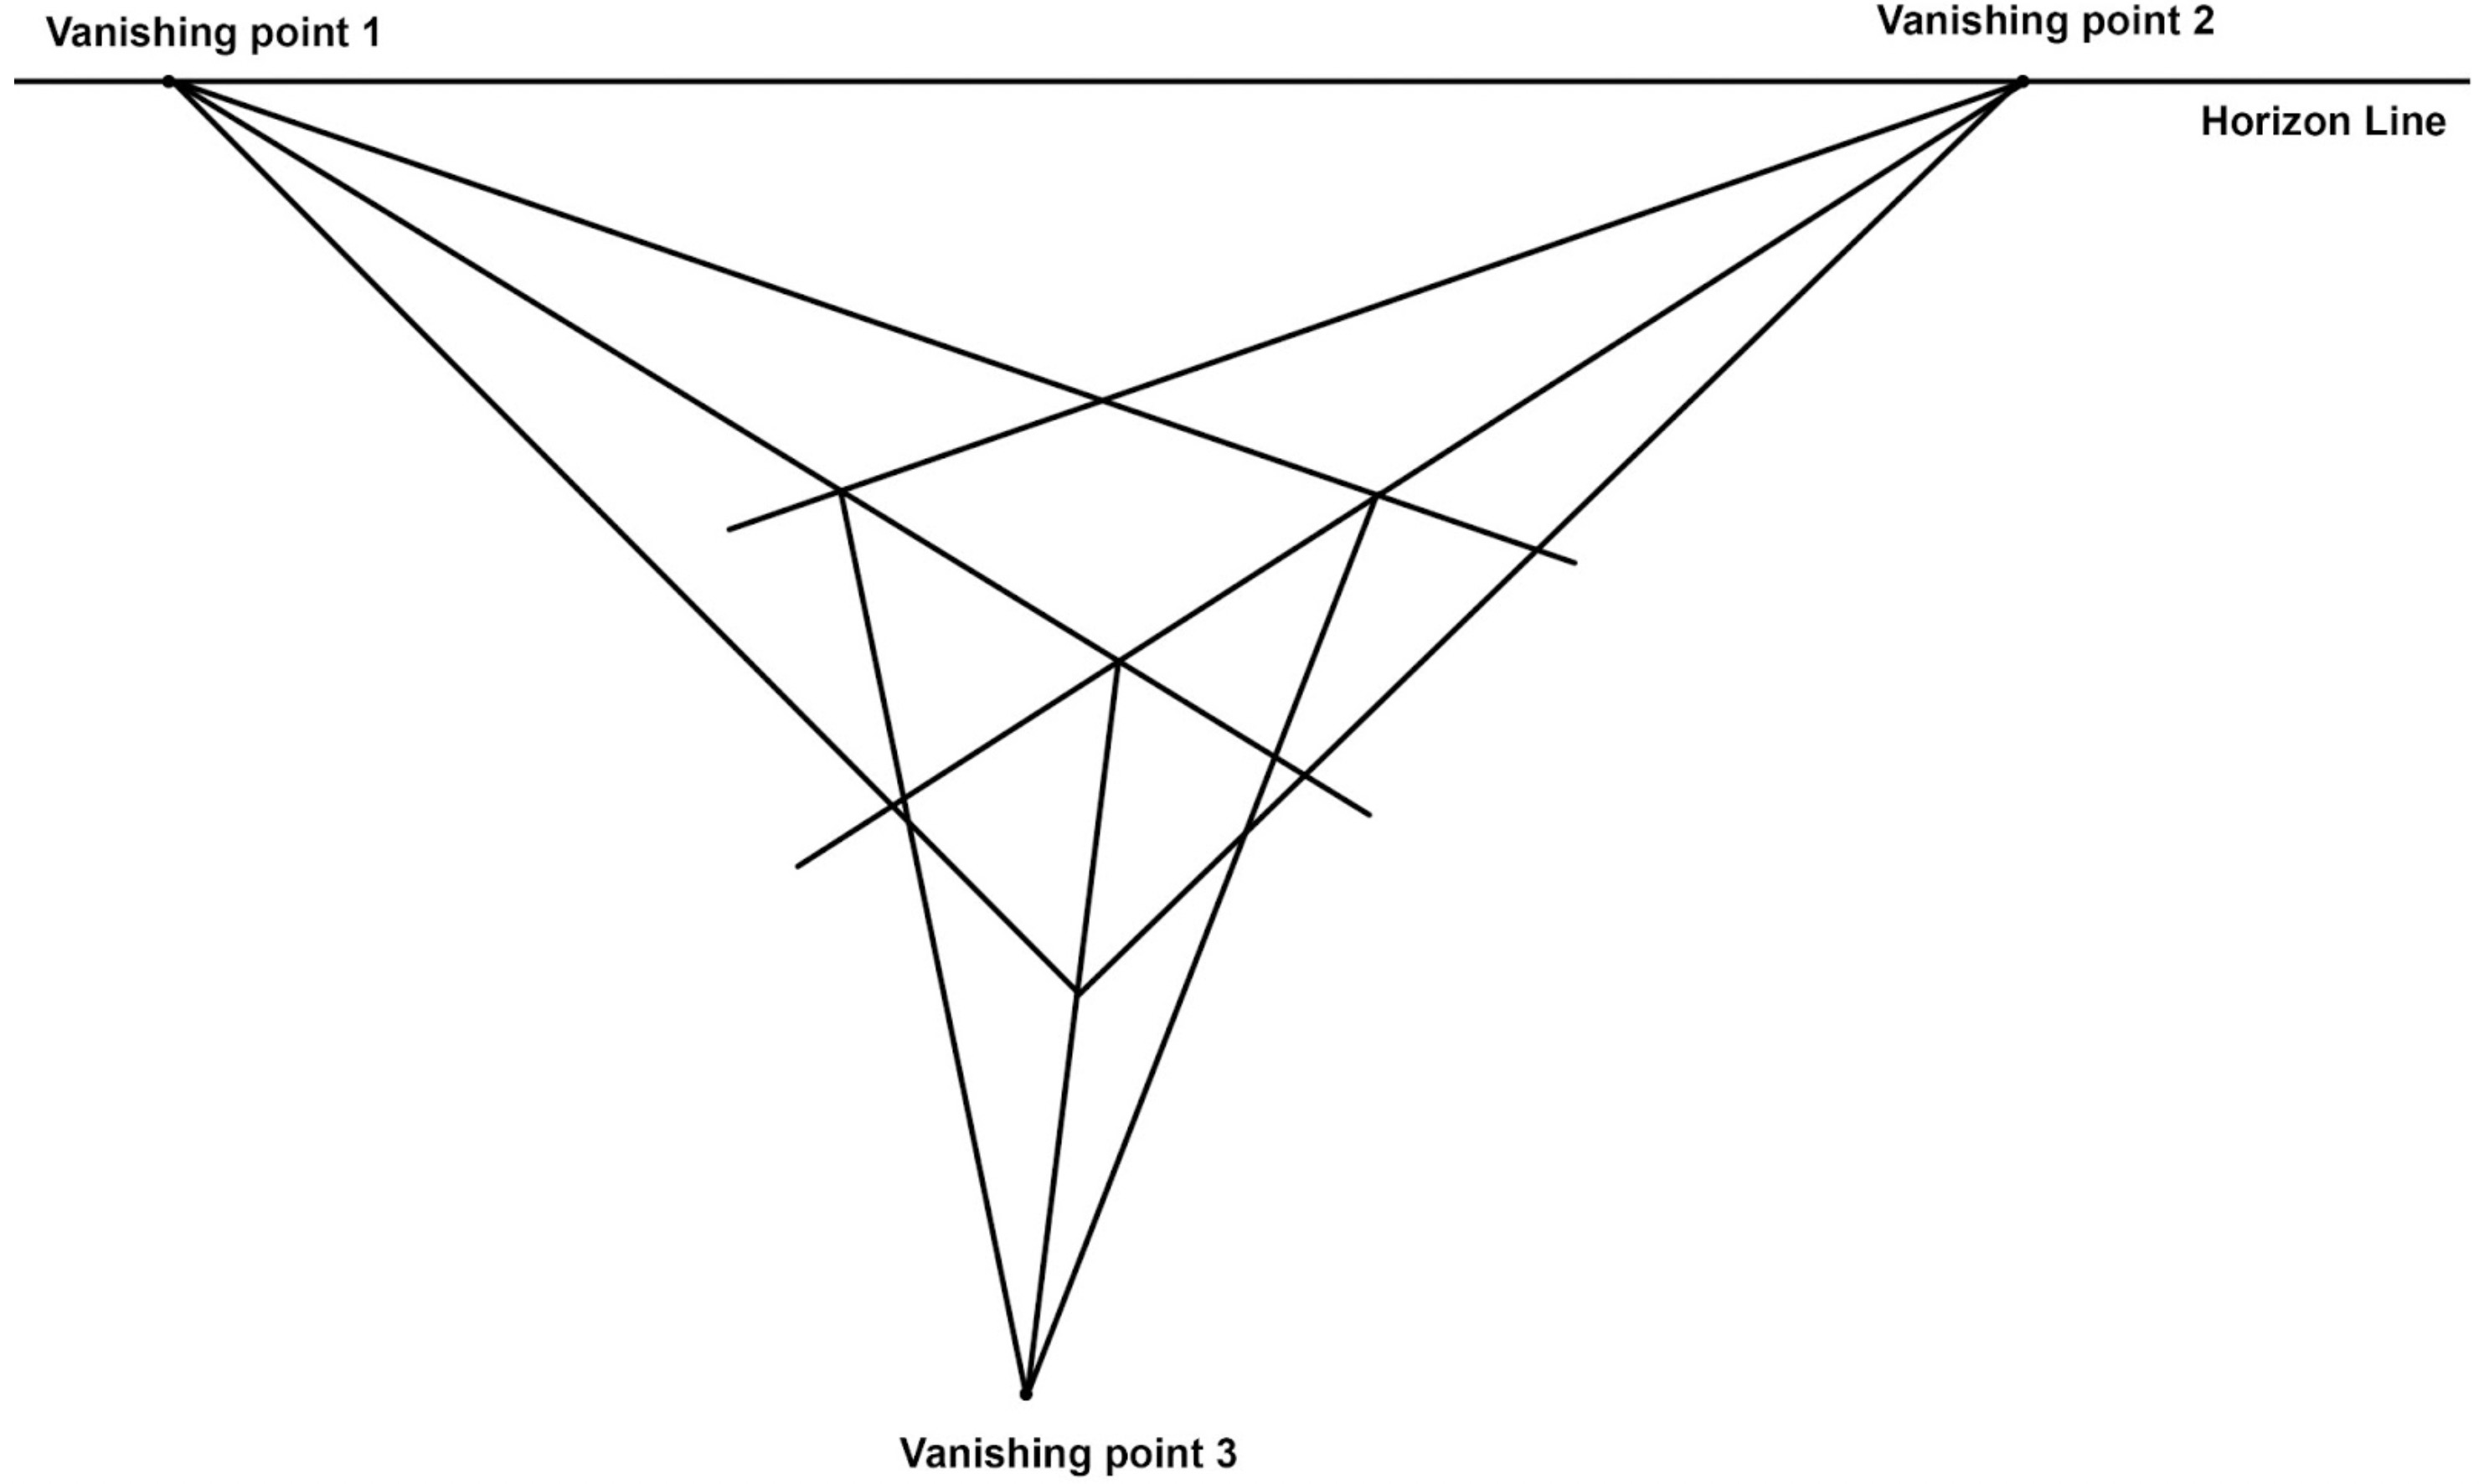
\includegraphics[width=0.5\linewidth]{cube.jpeg}
    \caption{Cube}
    \end{figure}
Each vanishing point is the point on the image corresponding to a point in 3D space at infinity of the form $(\mathbf{d}, 0) ^ {T}$, where $\mathbf{d}$ is a Euclidean vector with 3 coordinates expressing the direction of a cube edge. 
\begin{subparts}
    \subpart
    ** Show that the coordinates of a vanishing point $\mathbf{v}$ can be expressed as $\mathbf{v} = K R \mathbf{d}$, where $K$ is the intrinsic calibration matrix and $R$ is the rotation matrix between the camera and world coordinate system. Hence express an edge direction $\mathbf{d}$ as a function of K, R and $\mathbf{v}$. (Hint: Start from the $3\times4$ projection matrix equation in Ch 1)
    
    \begin{solution}
        Let $\mathbf{d}=(a, b, c) ^ {T}$, and apply the projection matrix to point at infinity in 3D space $x _ {\infty} = (a, b, c, 0) ^ {T}$:
        \begin{equation}
                    \begin{split}
            \mathbf{v} &= M x _ {\infty} = K \left[R \quad T\right] \left( \begin{array}{c}
                 a  \\
                 b  \\
                 c  \\
                 0
            \end{array} \right) \\
            &= K R \left( \begin{array}{c}
                 a  \\
                 b  \\
                 c  
            \end{array} \right) \\
            &= K R \mathbf{d}
        \end{split}
        \end{equation}
        Hence, the direction vector is:
        \begin{equation}
            \mathbf { d } = \frac { (KR) ^ { - 1 }   \mathbf{v}  } { \left\| (KR) ^ { - 1 }  \mathbf{v}  \right\| }
        \end{equation}
        
        
    \end{solution}
    
    \subpart
    ** The 3 directions of the cube edges are mutually perpendicular; therefore the dot product between any two directions is zero. Show that this condition leads to an equation in terms of the vanishing points and the unknown calibration matrix $K$. Note that such an equation can be written for each pair of the 3 vanishing points.
    
    \begin{solution}
        First, the angle between any two directions in the 3D space is given by the cosine rule:
        \begin{equation}
            \begin{aligned} \cos \theta & = \frac { \mathbf{d} _ { 1 } \cdot \mathbf{d} _ { 2 } } { \left\| \mathbf{d} _ { 1 } \right\| \left\| \mathbf{d} _ { 2 } \right\| } \\ & = \frac { v _ { 1 } ^ { T } \omega v _ { 2 } } { \sqrt { v _ { 1 } ^ { T } \omega v _ { 1 } } \sqrt { v _ { 2 } ^ { T } \omega v _ { 2 } } } \end{aligned}
        \end{equation}
        where $\omega = \left( (KR) (KR) ^ { T } \right) ^ { - 1 } = \left( K K ^ { T } \right) ^ { - 1 }$.
        
        As given, all the edges are mutually perpendicular, therefore $\cos \theta = 0$, and the equations given by these three vanishing points are:
        \begin{equation}
            v  _ { 1 } ^ { T  } \omega  v  _  2  = v  _ { 1 } ^ { T  } \omega  v  _  {3} = v  _ { 3 } ^ { T  } \omega  v  _  {3} =0
        \end{equation}
    \end{solution}
    
    \subpart
    *** Note that the derived equation above can be used to solve for K, but you are not required to explicitly propose a scheme for solving this equation. However, doing so will earn you bonus point.
    
    \begin{solution}
        In this setup, we have three constraints, but the unknown $K$ has five degrees of freedom. Hence, we could make assumption that the camera has zero-skew and square pixels to add two more constraints on it.
        
        Our original intrinsic matrix is given by:
        \begin{equation}
            K = \left[ \begin{array} { c c c } { \frac { - 1 } { s _ { x } } } & { k } & {  { o } _ { x } } \\ { 0 } & { \frac { - 1 } { S _ { y } } } & {  { o } _ { y } } \\ { 0 } & { 0 } & { 1 } \end{array} \right]
        \end{equation}
        
        By the additional constraints, it becomes:
        \[
            K = \left[ \begin{array} { c c c } { \alpha } & { 0 } & {  { o } _ { x } } \\ { 0 } & { \alpha } & {  { o } _ { y } } \\ { 0 } & { 0 } & { 1 } \end{array} \right]
        \]
        Therefore, with three equations, to solve three unknowns becomes possible. And by doing this we calibrate the camera with a single image!
    \end{solution}
\end{subparts}

\part
The projection of a scene point in world coordinates to pixel coordinates in an image can be represented using a camera projection matrix $P$ as follows:
\[
\left( \begin{array} { c } { s _ u } \\ { s _ v } \\ { s } \end{array} \right) = \left[ \begin{array} { l l l l } { p _ { 11 } } & { p _ { 12 } } & { p _ { 13 } } & { p _ { 14 } } \\ { p _ { 21 } } & { p _ { 22 } } & { p _ { 23 } } & { p _ { 24 } } \\ { p _ { 31 } } & { p _ { 32 } } & { p _ { 33 } } & { p _ { 34 } } \end{array} \right] \left( \begin{array} { c } { X _ { w } } \\ { Y _ { w } } \\ { Z _ { w } } \\ { 1 } \end{array} \right)
\]
\begin{subparts}
    \subpart
    * Given a set of lines in a scene that are all parallel to the world $X$-axis, what is the vanishing point, $(u, v)$, of these lines in the image? Can you conclude whether an infinite line in 3D space always yield an infinite line in the 2D image plane?
    
    \begin{solution}
        Let a point at infinity in 3D space $x_{\infty} = (1, 0, 0, 0) ^ {T}$.
        Apply the projection matrix $P$, we obtain the corresponding image point:
        \[
        \left( \begin{array} { c } { s _ u } \\ { s _ v } \\ { s } \end{array} \right) = \left( \begin{array} { c } { p_{11} } \\ { p_{21} } \\ { p_{31}} \end{array} \right)
        \]
        As we can observe, an infinite line in 3D space dons \textbf{not} necessarily yield an infinite line in 2D image plane, since the $s$ component may be non-zero. For example, if the projection is an affine transformation, the image line will be at infinity; however, is the projection is an projective transformation, the image line will not be at infinity.
    \end{solution}
    
    \subpart
    What is the significance of the image point (represented as a homogeneous 3-vector) given by the last column $(p _ {14}, p_ {24}, p_ {34})$ of $P$? That is,which world point gives rise to  $(p _ {14}, p_ {24}, p_ {34})$ ?
    
    \begin{solution}
        If the world point is $(0,0,0,1) ^ {T}$, the corresponding image point will be $(p _ {14}, p_ {24}, p_ {34})$. Actually is the image point of the plane at infinity $\Pi _ {\infty} = (0,0,0,1) ^ {T}$, and it's also referred as \textbf{horizon line}. 
    \end{solution}
    
    \subpart
    ** Consider the 1-dimensional right null-space of $P$, i.e., the 4-vector $\mathbf{C}$ such that $P \mathbf{C}=0$. In this case, the image point of $\mathbf{C}$ is $(0, 0, 0) ^ {T}$ which is not defined. What is the point $\mathbf{C}$ which possesses this property? Explain.
    
    \begin{solution}
        Point $\mathbf{C}$ should be the camera center.
        \begin{proof}
            Let $\mathbf{A}$ be an arbitrary point in the 3D space. A line can be formed by connecting point $\mathbf{A}$ and point $\mathbf{C}$. Points on this line can be described by:
            \begin{equation}
                \mathbf { X } ( \lambda ) = \lambda \mathbf { A } + ( 1 - \lambda ) \mathbf { C } , - \infty < \lambda < \infty
            \end{equation}
            Under the projection $ \mathbf { x } = P \mathbf { X }$, the image point on this line can be described by:
            \begin{equation}
                \mathbf { x } = P \mathbf { X } ( \lambda ) = \lambda \mathrm { P } \mathbf { A } + ( 1 - \lambda ) \underbrace { P \mathbf { C } } _ { = 0 } = \lambda \mathrm { P } \mathbf { A } , - \infty < \lambda < \infty
            \end{equation}
            Eq. (20) shows that all the points on this 3D line are mapped to the same point. Thus this line must go through the camera center. Additionally, since point $\mathbf{A}$ is arbitrary, to make sure the line goes through the camera center, point $\mathbf{C}$ must be the camera center.
        \end{proof}
    \end{solution}
\end{subparts} 

    \part
    The equation of a conics in inhomogeneous coordinates is given by $a x ^ { 2 } + b x y + c y ^ { 2 } + d x + e y + f  = 0$. 
    \begin{subparts}
        \subpart
        Homogenize this equation by the replacement $ x \rightarrow \frac{x_{1}}{x_{3}} $, $ y \rightarrow \frac{x_{2}}{x_{3}} $, and write down the homogeneous form. Finally, express this homogeneous form in the matrix form $\mathbf { x } ^ {  T  }  \mathrm { C }  \mathbf { x } = 0$, where $\mathrm { C }$ is symmetric. Write down the elements of the symmetric matrix $\mathrm { C }$.
        
        \begin{solution}
            In homogeneous coordinate, the conics equation becomes:
            \begin{equation}
                a x _ { 1 } ^ { 2 } + b x _ { 1 } x _ { 2 } + c x _ { 2 } ^ { 2 } + d x _ { 1 } x _ { 3 } + e x _ { 2 } x _ { 3 } + f x _ { 3 } ^ { 2 } = 0
            \end{equation}
            This can be written in matrix form:
            \begin{equation}
                \left( \begin{array} {c c c} {x _ {1}} & {x _ {2}} & {x _ {3}}  \end{array} \right) \left[ \begin{array} { c c c } { a } & { b / 2 } & { d / 2 } \\ { b / 2 } & { c } & { e / 2 } \\ { d / 2 } & { e / 2 } & { f } \end{array} \right] \left( \begin{array} {c} x _ {1} \\ x _ {2} \\ x _ {3} \end{array} \right) = 0
            \end{equation}
            So the symmetric conics matrix $\mathrm { C } = \left[ \begin{array} { c c c } { a } & { b / 2 } & { d / 2 } \\ { b / 2 } & { c } & { e / 2 } \\ { d / 2 } & { e / 2 } & { f } \end{array} \right]$.
        \end{solution}
        
        \subpart
        ** If $\mathrm { C }$ has the special form $\mathrm { C } = \mathbf{l} \mathbf{m} ^ {T} + \mathbf{m} \mathbf{l} ^ {T}$ , clearly $\mathrm { C }$ is symmetric and therefore represents a conic. Show that the vector $\mathbf{x} = \mathbf{l} \times \mathbf{m}$ is the null vector of $\mathrm { C }$. Since a null vector exists, $\mathrm { C }$ is a degenerate conic. Show in this degenerate case, $\mathrm { C }$ contains two lines $\mathbf{l}$ and $\mathbf{m}$, that is, show that the points on the lines $\mathbf{l}$ and $\mathbf{m}$ satisfy $\mathbf { x } ^ { T }   \mathrm{C}  \mathbf { x } = 0$.
        
        \begin{solution}
            We know that in homogeneous coordinate, $\mathbf{x} = \mathbf{l} \times \mathbf{m}$ means that $x$ is the intersection of lines $\mathbf{m}$ and $\mathbf{l}$. Thus we have:
            \begin{equation}
                \mathbf{m} ^ {T} \mathbf{x} = 0, \quad \mathbf{l} ^ {T} \mathbf{x} = 0
            \end{equation}
            Therefore, to show that $\mathbf{x}$ is the null vector of $\mathrm { C }$:
            \begin{equation}
                    \mathrm { C } \mathbf{x} = \mathbf{l} \mathbf{m} ^ {T} \mathbf{x} + \mathbf{m} \mathbf{l} ^ {T} \mathbf{x} = \mathbf{0}
            \end{equation}
            
            Since conic $\mathrm{C}$ has a null vector, the matrix $\mathrm{C}$ is not of full rank, and it is a degenerate conic. To show line $\mathbf{l}$ is on this conic, let $\mathbf{p}$ be any arbitrary point on line $\mathbf{l}$, we have $\mathbf{l} ^ {T} \mathbf{p} = \mathbf { p } ^ { T } \mathbf { l }  = 0$. To evaluate $\mathbf{p} ^ {T} \mathrm{C} \mathbf{p}$:
            \begin{equation}
                \mathbf { p } ^ { T } \mathrm { C } \mathbf { p } = \left( \mathbf { p } ^ { T } \mathbf { l } \right) \left( \mathbf { m } ^ { T } \mathbf { p } \right) + \left( \mathbf { p } ^ { T } \mathbf { m } \right) \left( \mathbf { l } ^ { T } \mathbf { p } \right) = 0
            \end{equation}
            This shows $\mathbf{p}$ is on this conic. Since $\mathbf{p}$ is any arbitrary point on line $\mathbf{l}$, line $\mathbf{l}$ is on this conic.
            
            Using the similar steps for line $\mathbf{m}$ ($\mathbf{m} ^ {T} \mathbf{p} = \mathbf { p } ^ { T } \mathbf { m }  = 0$), we can get the same result as Eq. (25). 
            
            Thus, we can conclude that this degenerate conic contains two lines $\mathbf{l}$ and $\mathbf{m}$, and their intersection is the null vector for conic matrix $\mathrm{C}$.
        \end{solution}
    \end{subparts}
    
    \part
    Given a set of two-dimensional points $(x,y)$ as follows (not listed here, can be found in $conics.txt$), write a Matlab routine to find the conics best (in the least squares sense) represented by these points, in terms of the parameters $a, b, c, d, e,$ and $f$, as formulated in Question $3(d)$.
    
    \begin{solution}
        Any point $(x _ {i} , y _ {i})$ on the conic should satisfy the conic equation:
        \begin{equation}
            a x _ {i} ^ { 2 } + b x _ {i} y _ {i} + c y _ {i} ^ { 2 } + d x _ {i} + e y _ {i} + f  = 0
        \end{equation}
        This can be written as:
        \begin{equation}
            \left( \begin{array} { l l l l l l } { x _ { i } ^ { 2 } } & { x _ { i } y _ { i } } & { y _ { i } ^ { 2 } } & { x _ { i } } & { y _ { i } } & { 1 } \end{array} \right) \mathbf { c } = 0
        \end{equation}
        where $\mathbf { c } = ( a , b , c , d , e , f ) ^ { T }$ is the conic $\mathrm{C}$ as a 6-vector. This becomes a least square problem of the form $Ax=0$. The Matlab routine as below will find the ``best" conic:
        \begin{lstlisting}
load conics.txt
c = fit_conic(conics);
x = conics(:,1);
y = conics(:,2);
scatter(x,y)
hold on
fimplicit(@(x,y) c(1)*x^2 + c(2)*x*y + c(3)*y^2 + c(4)*x + c(5)*y + c(6))
xlabel('x')
ylabel('y')

function c = fit_conic(pts)
    x = pts(:,1);
    y = pts(:,2);
    A = [x.^2, x.*y, y.^2, x, y, ones(size(x))];
    [U, S, V] = svd(A);
    c = V(:,length(V)); % last column is the null vector
end
        \end{lstlisting}
        The result is verified in by plotting the figure below.
    \end{solution}
    \begin{figure}[H]
        \centering
        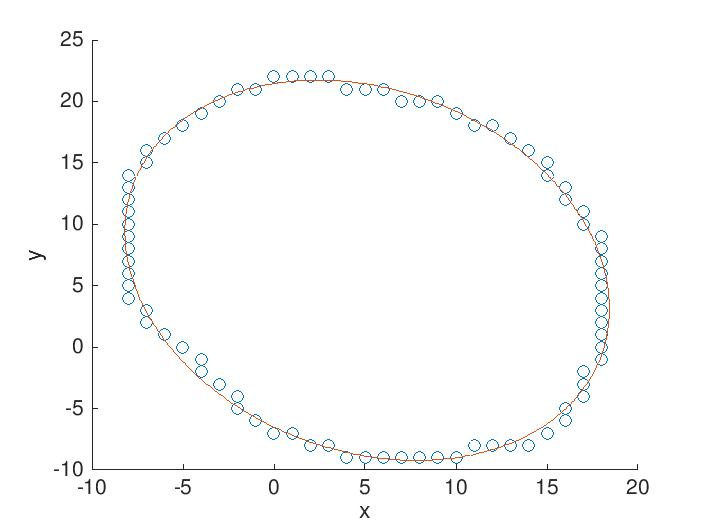
\includegraphics[width=0.6\linewidth]{conics_fitting.jpg}
    \end{figure}


\end{parts}
\end{questions}